\section{Methods}
\label{sec:methods}

\subsection{Category completeness and common calculation structure}

Each detailed IPPU category is assigned an IPCC notation key together with its available
activity data, methodological status, source provenance, materiality and remaining data
requirement. Emissions are calculated only when both the activity datum and the process
definition satisfy the relevant IPCC method. A production statistic may therefore establish
that an activity occurs without being sufficient to quantify its emissions. This distinction
keeps unavailable categories separate from reported zeros and excludes unrelated proxy data
from the national total.

All estimated categories use a common calculation structure containing the IPCC code,
activity value and unit, emission factor, source, method and uncertainty. Facility-level data
can replace aggregate national activity when they become available without changing the
underlying accounting method. The facility inventory receives emissions only when activity is
reported for the same plant boundary.

\begin{figure*}[htbp]
\centering
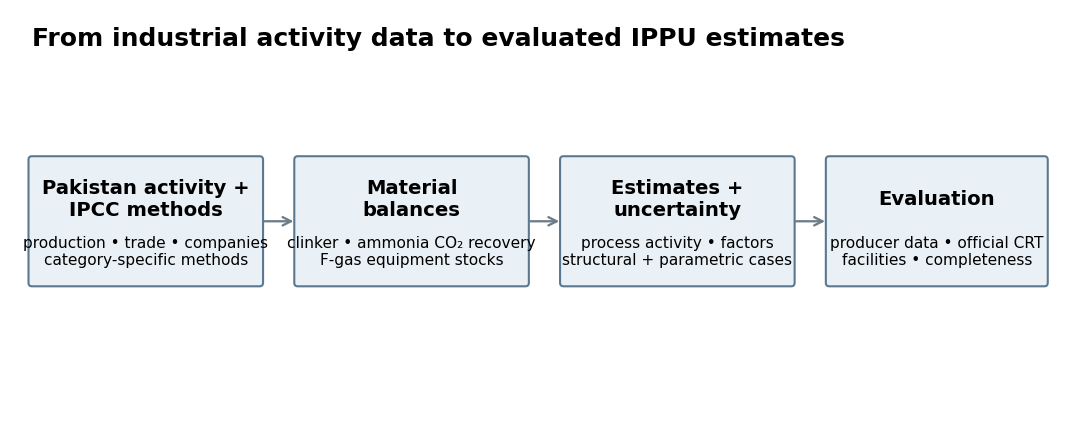
\includegraphics[width=0.94\textwidth]{ippu_framework.png}
\caption{Public inputs enter conserved material balances before category emissions are
calculated. Categories with insufficient evidence retain their notation keys and documented
data requirements.}
\label{fig:framework}
\end{figure*}

\subsection{Cement clinker balance}

For a fiscal year ending $y$, clinker contained in cement is
\begin{equation}
C^{\mathrm{cement}}_y=P^{\mathrm{cement}}_y f^{\mathrm{clinker}},
\end{equation}
and domestic clinker production is solved as
\begin{equation}
C^{\mathrm{production}}_y=C^{\mathrm{cement}}_y-I_y+X_y+\Delta S_y,
\label{eq:clinkerbalance}
\end{equation}
where $I$ and $X$ are clinker imports and exports and $\Delta S$ is the stock increase. This is
the sign convention implied by the IPCC Tier~1 worksheet: production plus imports minus
exports and stock increase equals clinker ground into cement \citep{ipcc2006ippu}. No public
stock series was identified, so $\Delta S=0$ in the reference configuration and stock change
remains an explicit data gap.

Process \COtwo{} is
\begin{equation}
E_{\COtwo{},y}=C^{\mathrm{production}}_y\,\mathrm{EF}_{\mathrm{clinker}},
\end{equation}
with an IPCC default factor of \SI{0.52}{\tonne} \COtwo{} per tonne of clinker. The estimate
covers calcination only. Kiln fuel belongs to Energy 1.A.2 and will be linked through the
shared facility inventory rather than included in 2.A.1.

\subsection{Structural and parametric uncertainty}

The source audit removes the apparent activity-source choice for FY2023--24: QIM and SBP agree
on \SI{39.566}{\mega\tonne}, while 48.011 Mt belongs to FY2021--22. Observed clinker trade is
required by Equation~\ref{eq:clinkerbalance} and is included in every valid current model.
The remaining declared structural choice is the clinker fraction, evaluated at 0.75 and 0.95.
Two no-trade calculations are retained separately as historical method benchmarks: one uses
the correct FY2023--24 activity to isolate trade omission, and the original result combines
trade omission with the superseded period tag. Neither enters the valid structural range.

Within both valid configurations, a seeded 10,000-iteration Monte Carlo samples bounded
triangular distributions for cement activity ($\pm5\%$), imports and exports ($\pm10\%$), and
the clinker factor ($\pm8\%$). The clinker fraction is fixed within each structural
configuration. We report conditional P2.5, median and P97.5 values rather than merging
discrete source/method choices into one probability interval.

For calendar 2022, the same equation is evaluated with twelve QIM monthly observations and
calendar-year clinker imports and exports. This makes the comparison with Pakistan's 2022 CRT
period-matched; the clinker fraction and zero stock change remain structural assumptions.

\subsection{Official-reporting audit}

The CRT audit extracts the native category cells rather than transcribing the published total.
For every numeric background row and gas, final emissions are reconstructed as
\begin{equation}
E^{\mathrm{final}}=A\times \mathrm{IEF}+R,
\end{equation}
where recovery $R$ is reported as a negative quantity. This treatment is important for
ammonia, where gross process \COtwo{} is partly recovered for downstream use. Arithmetic
closure tests the workbook; comparison with public evidence tests its activity, factor and
boundary choices.

\subsection{Spatial and temporal products}

The current cement provincial allocation preserves the legacy cement/limestone proxy only so
that downstream national and province tables remain reconciled. Its former Punjab activity
anchor is no longer treated as period-matched. Industrial
process emissions are point sources, so the target product is a facility ledger that
reconciles plant, district, province and national totals. Thirty-four facilities have been
identified; \num{24} carry resolved coordinates---one independently verified site geocode,
seven from named OSM industrial polygon centroids and \num{16} from the Global Energy
Monitor cement tracker, each point-in-polygon verified against
its census district at build---and the remaining \num{10} are located only to their reported
locality. Where both registers place the same works,
\texttt{outputs/ippu\_facility\_coordinate\_agreement.csv} records the separation: eight
sites are placed independently by OpenStreetMap and by the tracker and agree to within
\SIrange{0.024}{0.744}{\kilo\metre}. The file's other eleven rows are not evidence and say
so---those coordinates came from the tracker in the first place, so their distance to it is
zero and the comparison is a register against itself. Company-wide activity is assigned among plants only when
plant-specific evidence is available. Spatial and historical products are therefore reported
only where the required facility- or year-specific activity data have been assembled. A
1990--2024 coverage table records the remaining years as unavailable.
